\documentclass[12pt,
border=1pt]{standalone}
\usepackage{pgfplots}
\usepackage{amsmath}
\usepackage{amssymb}

\pgfplotsset{compat=newest,
	width=6cm, height=5cm,
	xtick pos=left, ytick pos=left,
	%            scaled x ticks=real:1e-6,
}
% Kernel 2 FP64
\begin{document}
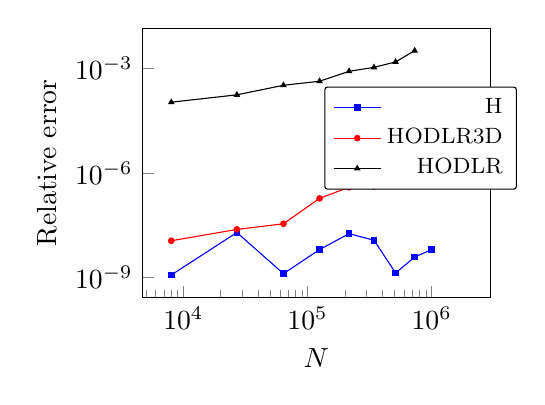
\begin{tikzpicture}[every mark/.append style={mark size=1pt}]
	\begin{axis}[xlabel={$N$},
	ylabel={Relative error},
%		legend pos=south east,
		legend style={
                at={(0.8,0.4)},
               anchor=south,
               legend columns=1,
               cells={anchor=east},
              font=\footnotesize,
               rounded corners=1pt,
               },
		xmode = log,
	    ymode = log,
	   % xmin = 1e3,
	   % xmax = 1e6,
	   % ymin = 1e-10,
	   % ymax = 1e-0,
	   % xtick={1e-10, 1e-8, 1e-6,  1e-4,  1e-2},
	   % ytick={1e-8, 1e-6,  1e-4,  1e-2, 1e-0}
		]
		
		\addplot[
		color=blue,
		mark=square*,
		] coordinates {
(8000,1.199520e-09)
(27000,1.981540e-08)
(64000,1.308370e-09)
(125000,6.399840e-09)
(216000,1.833530e-08)
(343000,1.188450e-08)
(512000,1.372290e-09)
(729000,3.910950e-09)
(1000000,6.425530e-09)
		};
		\addplot[
		color=red,
		mark=*,
		] coordinates {
(8000,1.147650e-08)
(27000,2.427980e-08)
(64000,3.523860e-08)
(125000,1.886480e-07)
(216000,3.926220e-07)
(343000,4.130920e-07)
(512000,7.718360e-07)
(729000,8.874070e-07)
(1000000,1.656790e-06)
(1331000,1.254110e-06)
(1728000,2.015970e-06)
		};
\addplot[
		color=black,
		mark=triangle*,
		] coordinates {
(8000,1.080530e-04)
(27000,1.757390e-04)
(64000,3.301860e-04)
(125000,4.310950e-04)
(216000,8.307520e-04)
(343000,1.077500e-03)
(512000,1.544970e-03)
(729000,3.248470e-03)
		};
% 		\addplot[mark=none, black, dashed][
% 		domain = 8000:512000,
% 		] {(pow(10,0.2)*pow(x,2/3)};
		\legend{H, HODLR3D, HODLR}	
		\end{axis}
\end{tikzpicture}
\end{document}